\titledquestion{Binary Tree Practice}
\begin{parts}

\part[2] Consider the Binary Search Tree (BST) $T$ shown below, which satisfies the BST property (where each node's key is the integer value itself) but is not height-balanced. Identify all nodes that are not height-balanced.

\begin{center}
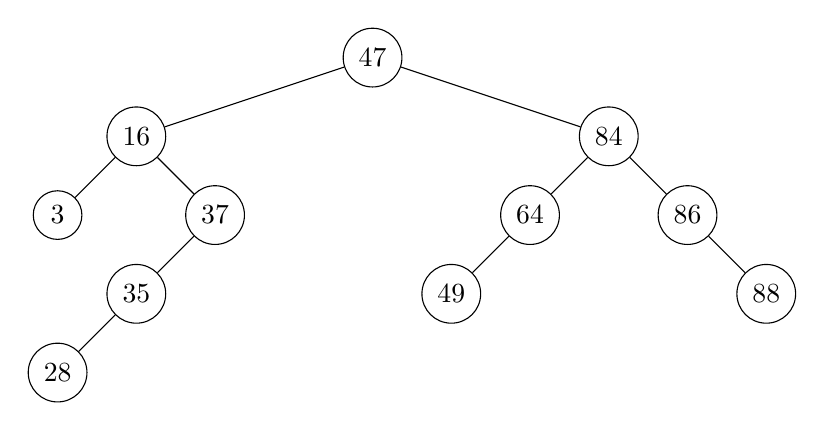
\begin{tikzpicture}[level distance=1cm,
            level 1/.style={sibling distance=2cm},
            level 2/.style={sibling distance=2cm},
            level 3/.style={sibling distance=2cm},
            every node/.style = {draw, circle}]
\node {47}
    child {node {16}
        child {node {3}}
        child {
            node {37}
            child {
                node {35}
                child { node {28} }
                child { edge from parent[draw=none] }
            }
            child { edge from parent[draw=none] }
        }
    }
    child { edge from parent[draw=none] }
    child { edge from parent[draw=none] }
    child {node {84}
        child {
            node {64}
            child { node {49} }
            child { edge from parent[draw=none] }
        }
        child {
            node {86}
            child { edge from parent[draw=none] }
            child { node {88} } 
        }
    };

\end{tikzpicture}
\end{center}

\begin{solution}
    \vspace{15pt}
\end{solution}

\part[5] Perform the following insertions and deletions, one after another in sequence on $T$, by adding or removing a leaf while maintaining the binary search tree property (a key may need to be swapped down into a leaf). For this part, do not use rotations to balance the tree. Draw the modified tree after each operation:
\begin{center}
    \texttt{T.insert(2)} \\
    \texttt{T.delete(49)} \\
    \texttt{T.delete(35)} \\
    \texttt{T.insert(85)} \\
    \texttt{T.delete(84)} \\
\end{center}

\begin{solution}
    \vspace{2.5in}

\end{solution}

\begin{solution}
    \vspace{8in}

\end{solution}

\end{parts}
